\chapter{Examples}

\section{Example 1: secondary channel along the Nederrijn}

For this first example, we compare the results of \dfastmi with the results of a morphological simulation using Delft3D-FLOW.
For consistency the \dfastmi analysis was performed using the hydrodynamic results of Delft3D-FLOW\footnote{Since \dfastmi expects \dflowfm results in netCDF UGRID format, the results were converted to the appropriate file format by means of \texttt{sim2ugrid}, see \autoref{Chp:Sim2Ugrid}.}.

For this analysis, the Nederrijn grid of the DVR model has been used.
The intervention concerns a secondary channel planned in the Palmerswaard which is located at Rkm 910-912 in the reach upstream of the Amerongen barrier at Rkm 922.
The reference model is based on the Baseline schematization ‘rijn-beno18\_5-v1’.
Since the DVR model was too coarse to represent the actual secondary channel, a combination of flow extraction (at Rkm 910.5) and insertion (at Rkm 912) was used to represent the side channel.

\begin{figure}
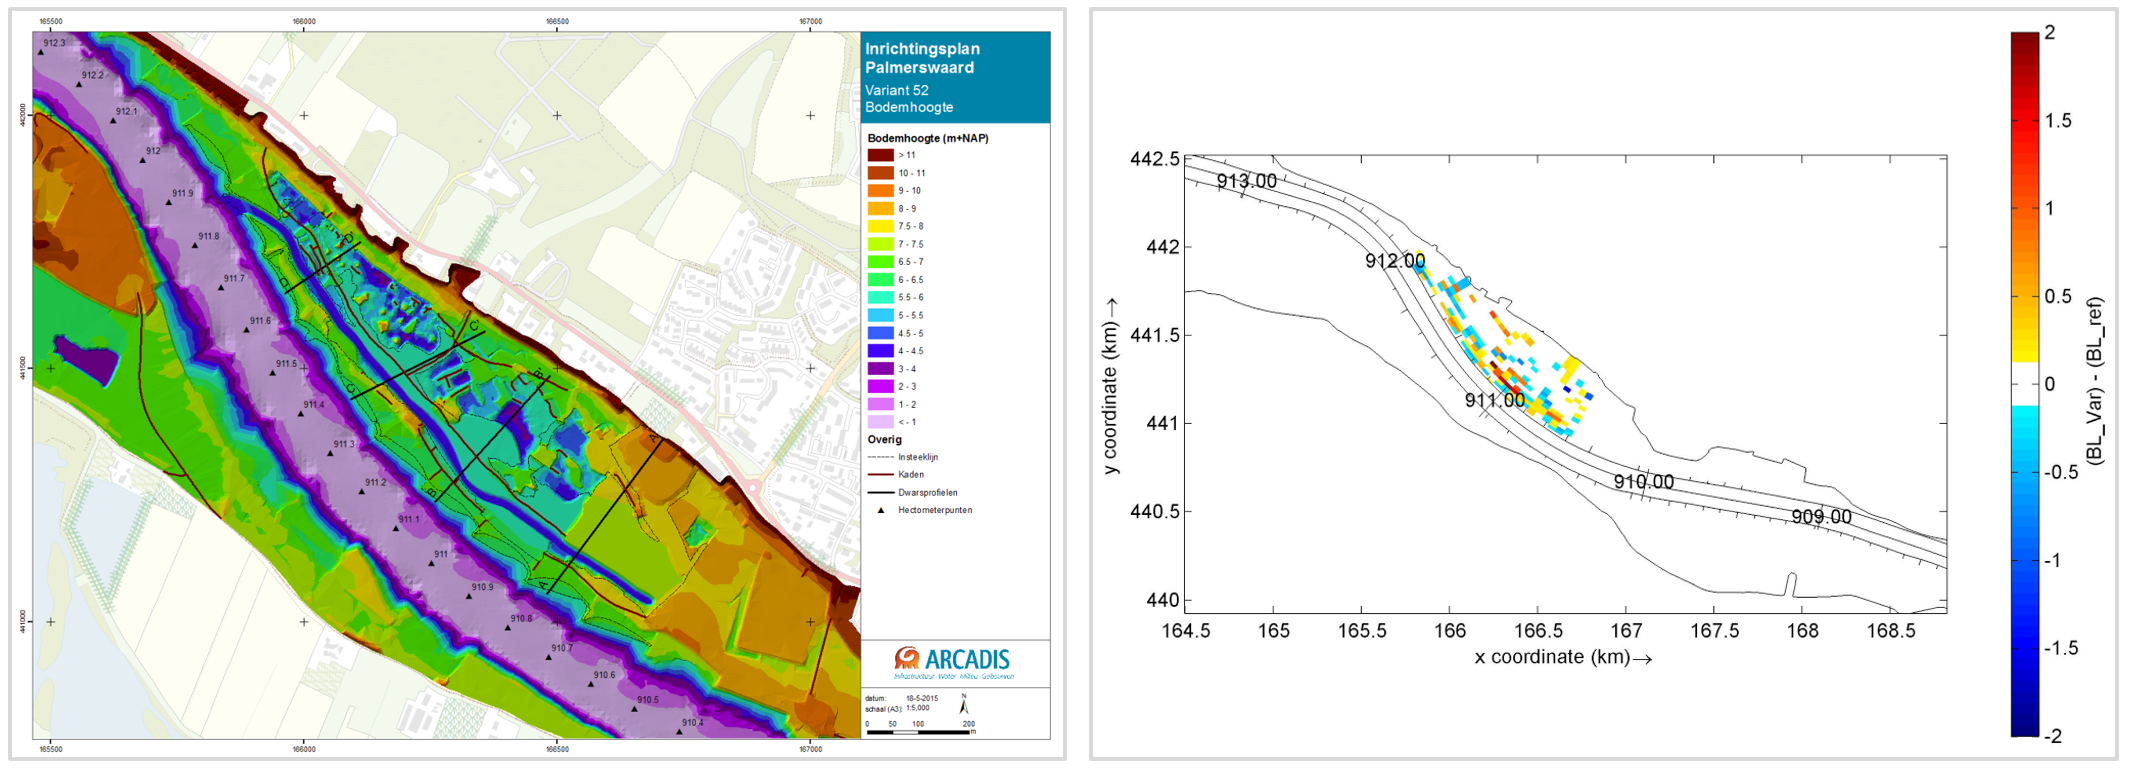
\includegraphics[width=\columnwidth]{figures/Palmerswaard_proj.png}
\caption{Side channel design (left) and initial representation on the grid (right).}
\label{Palmers_proj}
\end{figure}

Since the intervention is located on the Rhine branches, the new \dfastmi method requires the input of simulation results for 6 steady discharges: 1300, 2000, 3000, 4000, 6000, and \SI{8000}{\metre\cubed\per\second} at Lobith.
However, since the intervention is located in the backwater curve of the Amerongen barrier which is closed at discharges below \SI{1500}{\metre\cubed\per\second} causing largely stagnant flow conditions, the lowest discharge isn't relevant for this case.
Hence, \dfmi asks for the results of 10 simulations (5 discharges with and without intervention), see \autoref{Palmers_empty}.
After specifying all input files, the dialog will look like \autoref{Palmers_config} and if you save the configuration, the file will look as follows:

\begin{figure}
\center
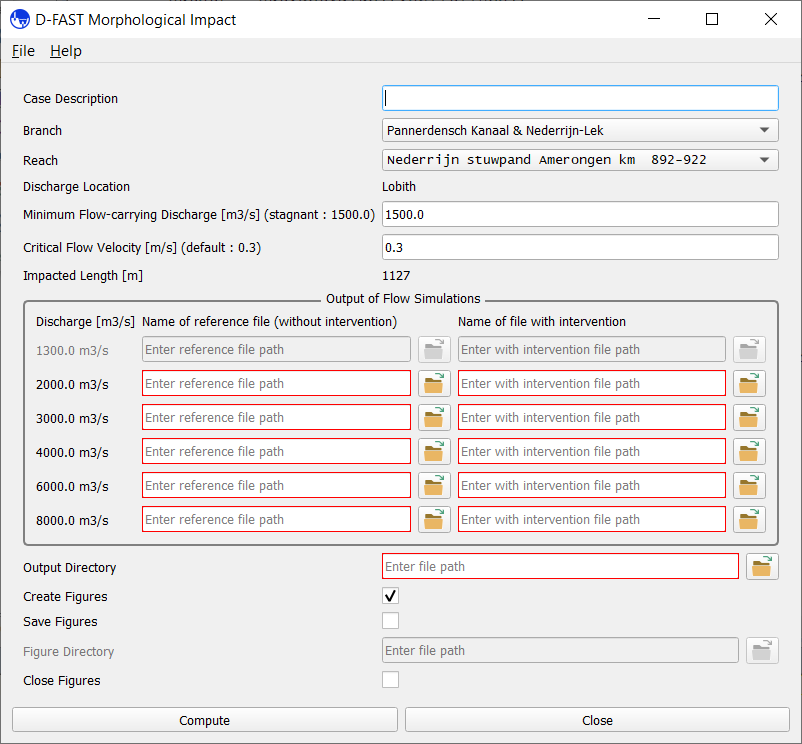
\includegraphics[width=11cm]{figures/Palmerswaard_empty.png}
\caption{Initial \dfmi screen after selecting the appropriate branch and reach.}
\label{Palmers_empty}
\end{figure}

\begin{figure}
\center
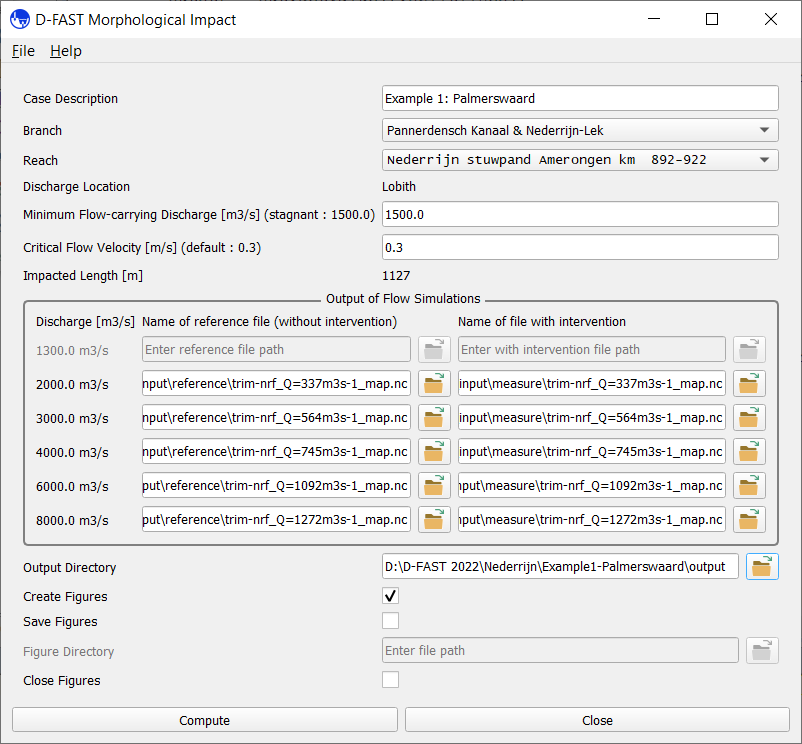
\includegraphics[width=11cm]{figures/Palmerswaard_config.png}
\caption{\dfmi screen after specifying all files.}
\label{Palmers_config}
\end{figure}

\verbfilenobox[\scriptsize]{figures/example1.cfg}

The \dfmi analysis is performed when you click on the \button{Compute} button.
The program will show a message that the analysis has successfully ended, and that a report.txt file has been written to the output folder.
Furthermore, since we have selected the "Create Figures" option, it will create a rudimentary overview picture of the change in the year-averaged equilibrium bed level that the result of the intervention.
The initial view will cover the whole model area as shown in \autoref{Palmers_fig}.
You can zoom in on the area of interest as shown in \autoref{Palmers_fig_zoomed}.
See \autoref{Sec:FigNavigation} for navigating these figures.
The content of the report file is shown below:

\begin{figure}
\center
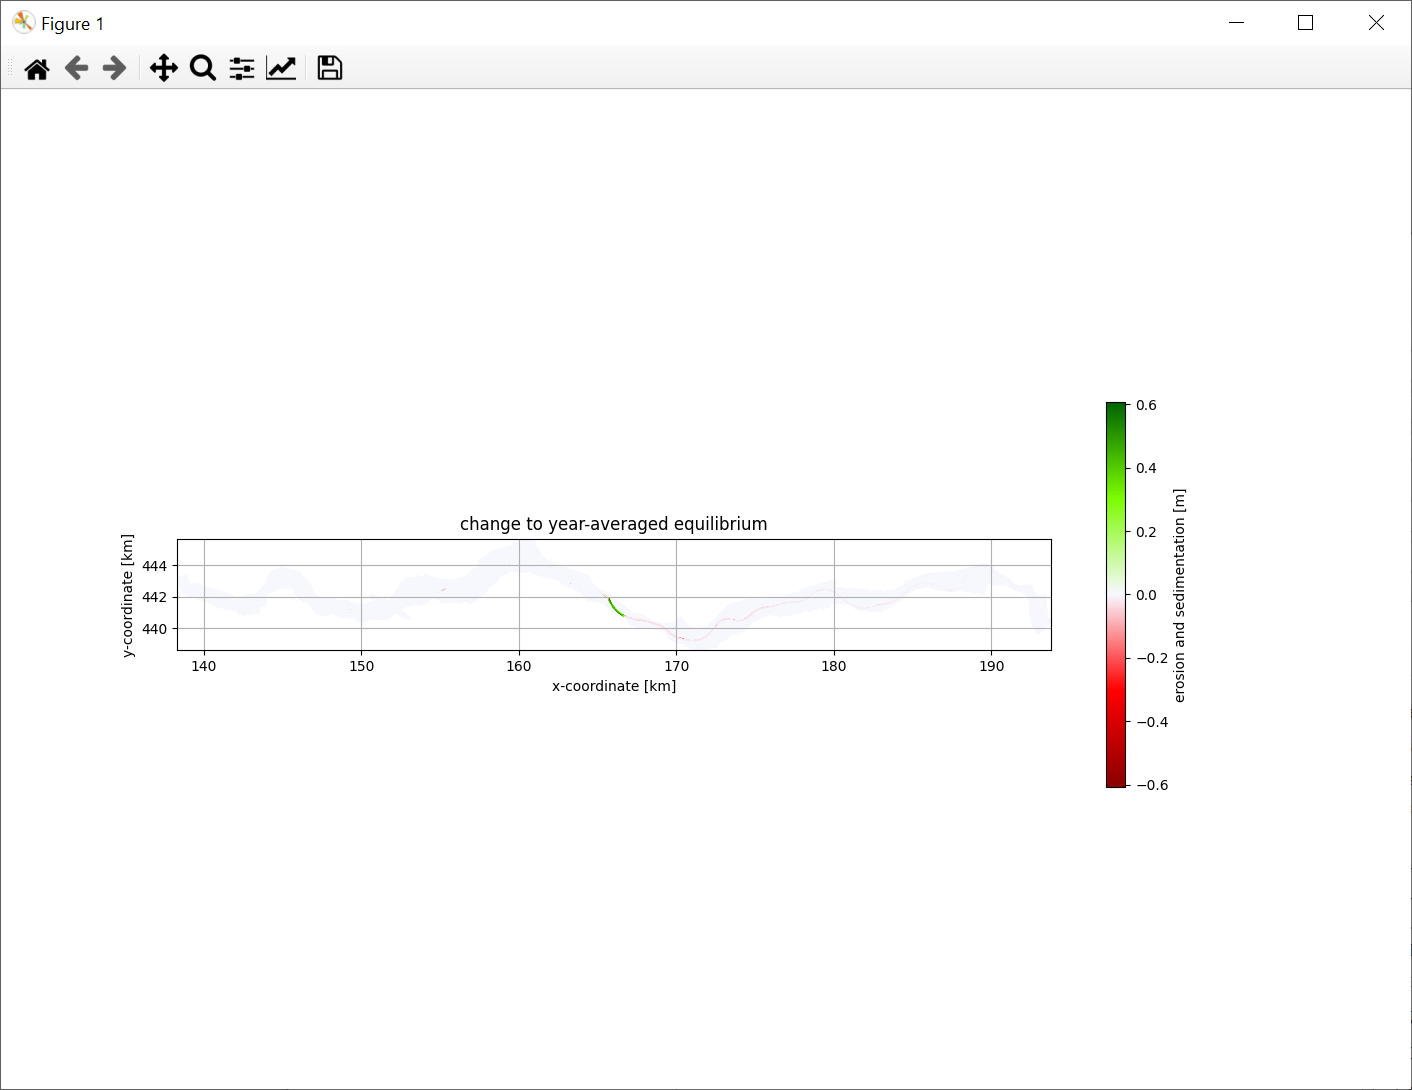
\includegraphics[width=\textwidth]{figures/Palmerswaard_fig.png}
\caption{Initial view of the analysis results.}
\label{Palmers_fig}
\end{figure}

\begin{figure}
\center
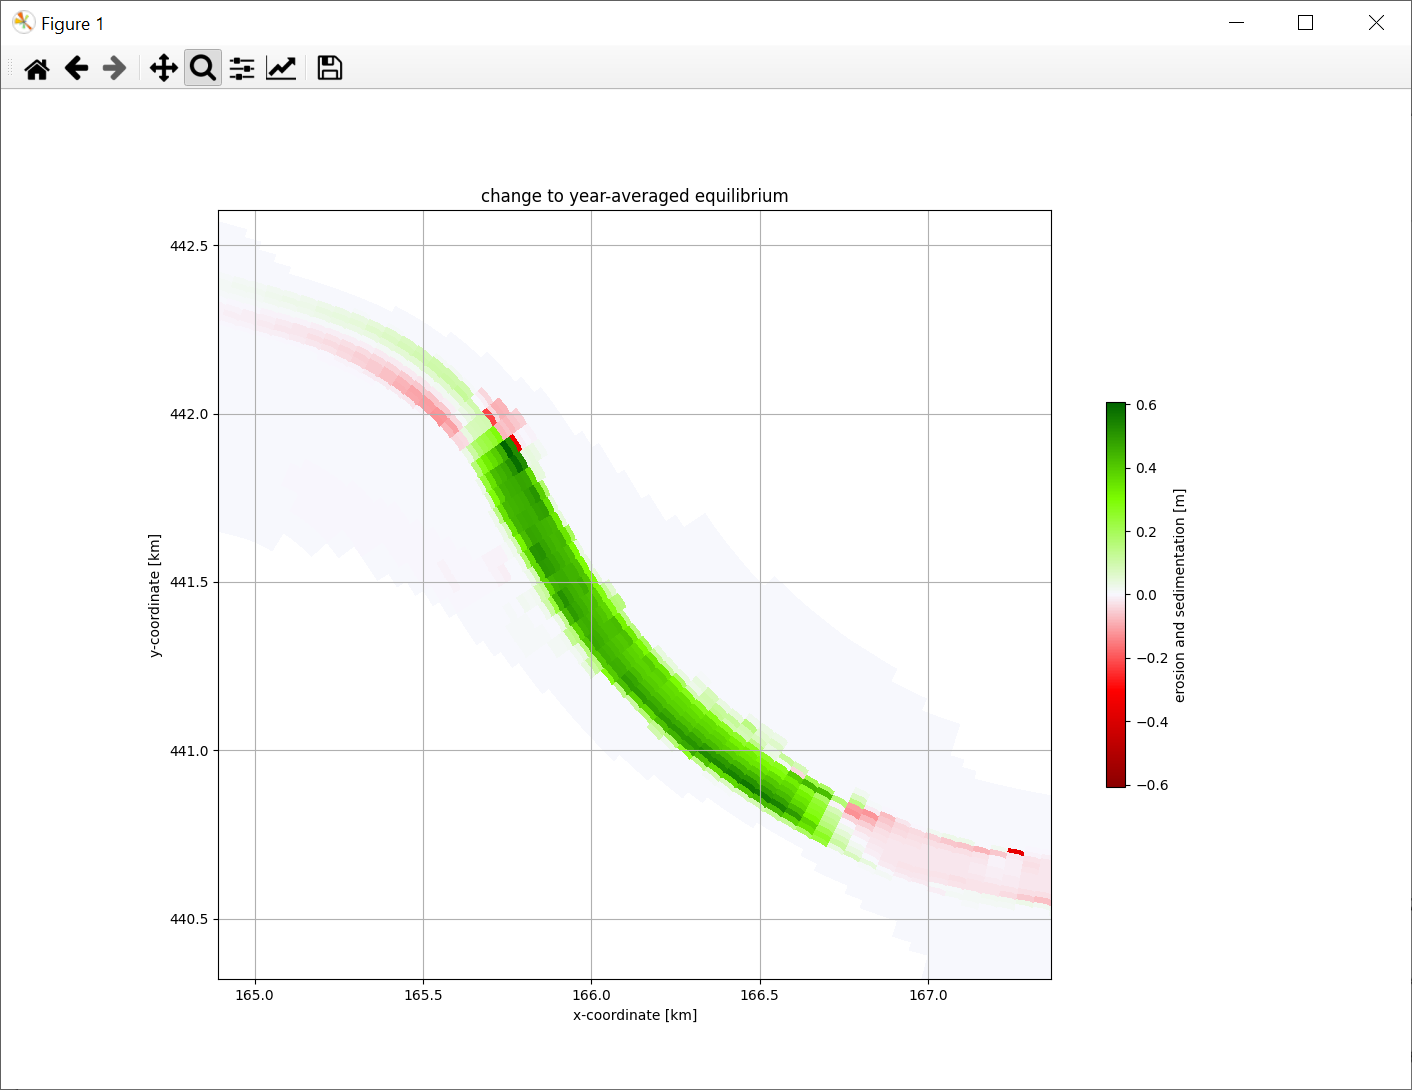
\includegraphics[width=\textwidth]{figures/Palmerswaard_fig_zoomed.png}
\caption{Zoomed view of the analysis results.}
\label{Palmers_fig_zoomed}
\end{figure}

\verbfilenobox[\scriptsize]{figures/example1_report.txt}

\autoref{Palmers_mor} shows the results of a reference morphology simulation using Delft3D 4 (for details, see \citet{GiriJagers2022}).
The figure shows the morphological evolution of the Delft3D simulation.
The overall \dfastmi results compare well with the long term (12yr) Delft3D simulation although the asymmetry downstream of the main sedimentation patch differs.

\begin{figure}[H]
\center
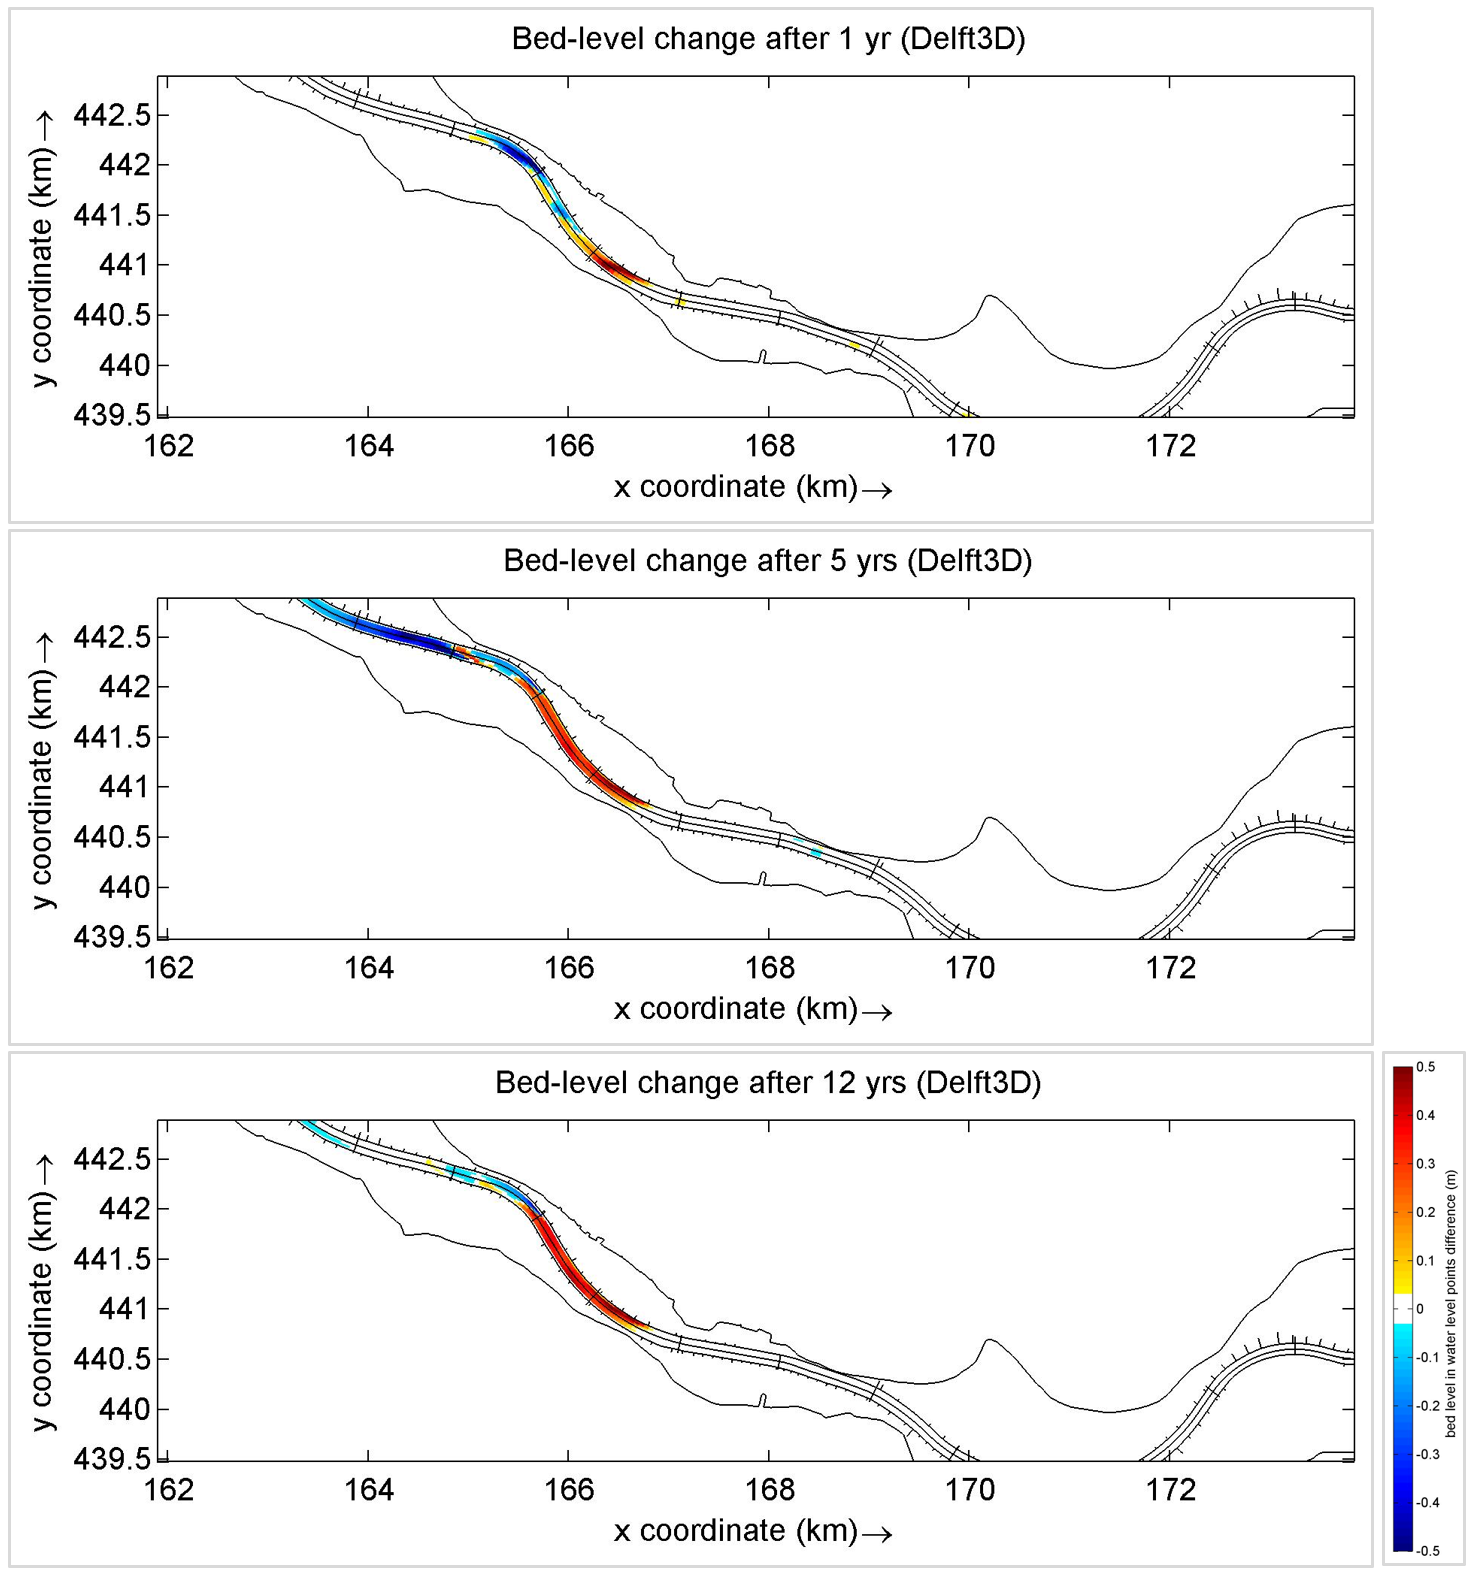
\includegraphics[width=\textwidth]{figures/Palmers_mor.png}
\caption{The bed-level difference between the variant and the reference after 1, 5 and 12 years of morphological simulation.}
\label{Palmers_mor}
\end{figure}


\section{Example 2: secondary channel along the Pannerdensch Kanaal}

For this second example, we follow the same approach as example 1: we compare the results of \dfastmi with the results of a morphological simulation using Delft3D-FLOW.
The model was based on the DVR model, but the domain was reduced to focus mainly on the Pannerdensch Kanaal \citep{BomLeeuwen2020}.
Because of the two bifurcations upstream and downstream, it still included parts of all the branches (Bovenrijn, Pannerdensch Kanaal, Waal, Nederrijn and IJssel).
Only results for the Pannerdensch Kanaal will be presented here.

The intervention concerns a secondary channel `green river' implemented along the right bank at Rkm 871-872 just downstream of Pannerden.
The reference model is based on the Baseline schematization ‘rijn-beno18\_5-v1’.
Again, a combination of flow extraction and insertion was used to represent the side channel because the secondary channel wasn't represented accurately on the grid.

\begin{figure}
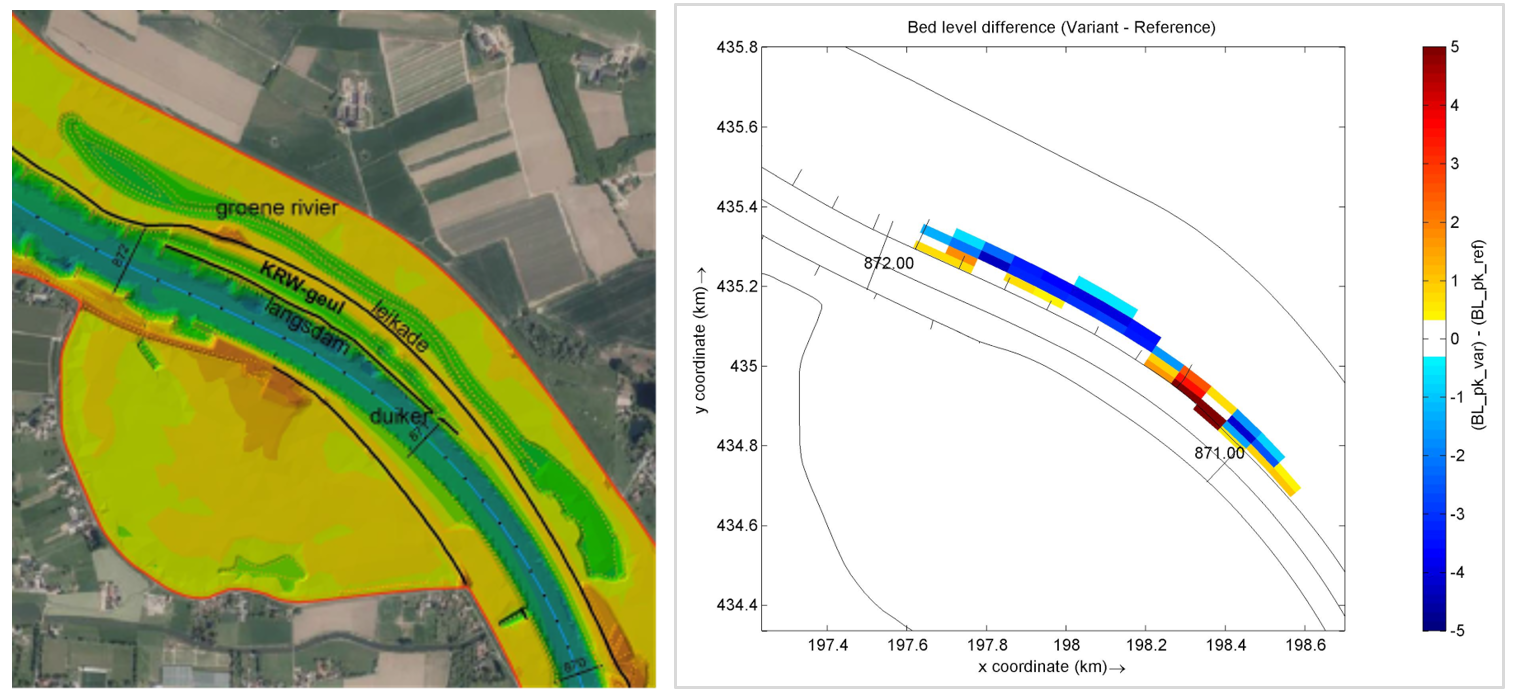
\includegraphics[width=\columnwidth]{figures/Pannerden_proj.png}
\caption{Side channel design (left) and initial representation on the grid (right).}
\label{Pannerden_proj}
\end{figure}

Since the intervention is located on the Rhine branches, the new \dfastmi method requires the input of simulation results for 6 steady discharges: 1300, 2000, 3000, 4000, 6000, and \SI{8000}{\metre\cubed\per\second} at Lobith.
Contrary to example 1, the lowest discharge is relevant for this case.
Hence, \dfmi asks for the results of 12 simulations (6 discharges with and without intervention).
After specifying all input files, the dialog will look like \autoref{Pannerden_config} and if you save the configuration, the file will look as follows:

\begin{figure}
\center
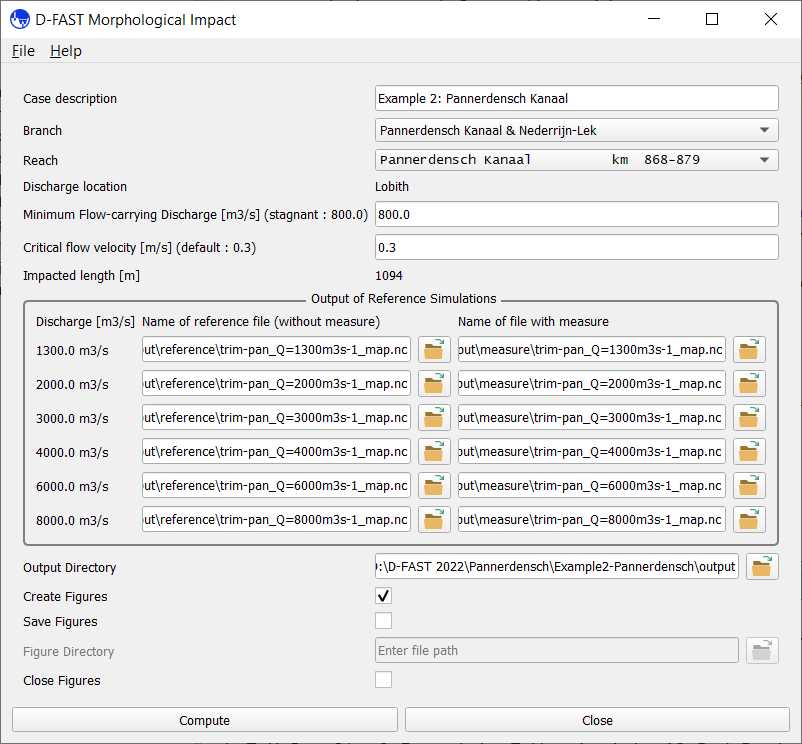
\includegraphics[width=11cm]{figures/Pannerden_config.png}
\caption{\dfmi screen after specifying all files.}
\label{Pannerden_config}
\end{figure}

\verbfilenobox[\scriptsize]{figures/example2.cfg}

The \dfmi analysis is performed when you click on the \button{Compute} button.
The program will show a message that the analysis has successfully ended, and that a report.txt file has been written to the output folder.
Furthermore, since we have selected the "Create Figures" option, it will create a rudimentary overview picture of the change in the year-averaged equilibrium bed level that the result of the intervention.
A zoomed-in version of that figure is shown in \autoref{Pannerden_fig_zoomed}.
See \autoref{Sec:FigNavigation} for navigating these figures.
The content of the report file is shown below:

\begin{figure}
\center
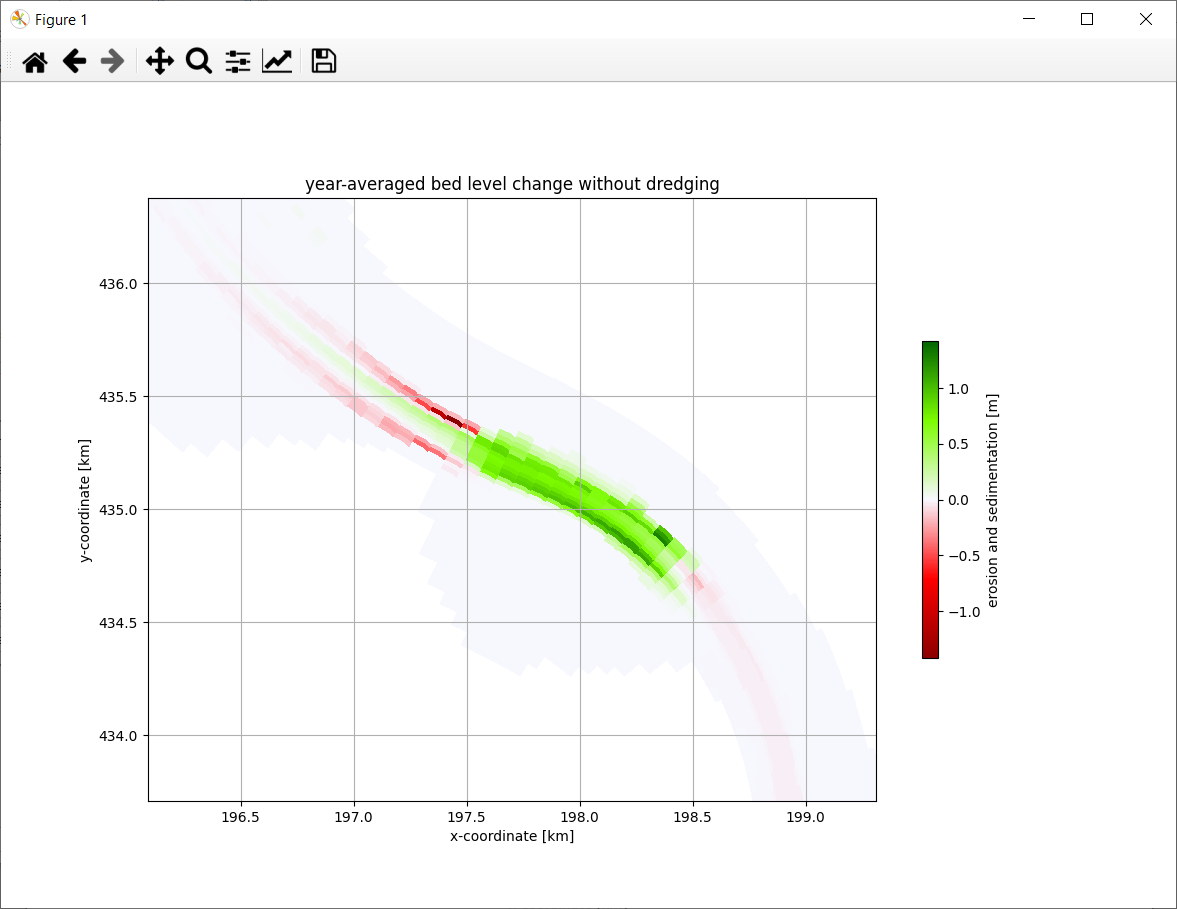
\includegraphics[width=\textwidth]{figures/Pannerden_fig_zoomed.png}
\caption{Zoomed view of the analysis results.}
\label{Pannerden_fig_zoomed}
\end{figure}

\verbfilenobox[\scriptsize]{figures/example2_report.txt}

\autoref{Pannerden_mor} shows the results of a reference morphology simulation using Delft3D 4 (for details, see \citet{GiriJagers2022}).
The figure shows the morphological evolution of the Delft3D simulation.
The overall \dfastmi results compare well with the long term (15yr) Delft3D simulation although \dfmi suggests sedimentation in the centre of the channel downstream of the main sedimentation area whereas the morphological simulation doesn't show that behaviour.

\begin{figure}[H]
\center
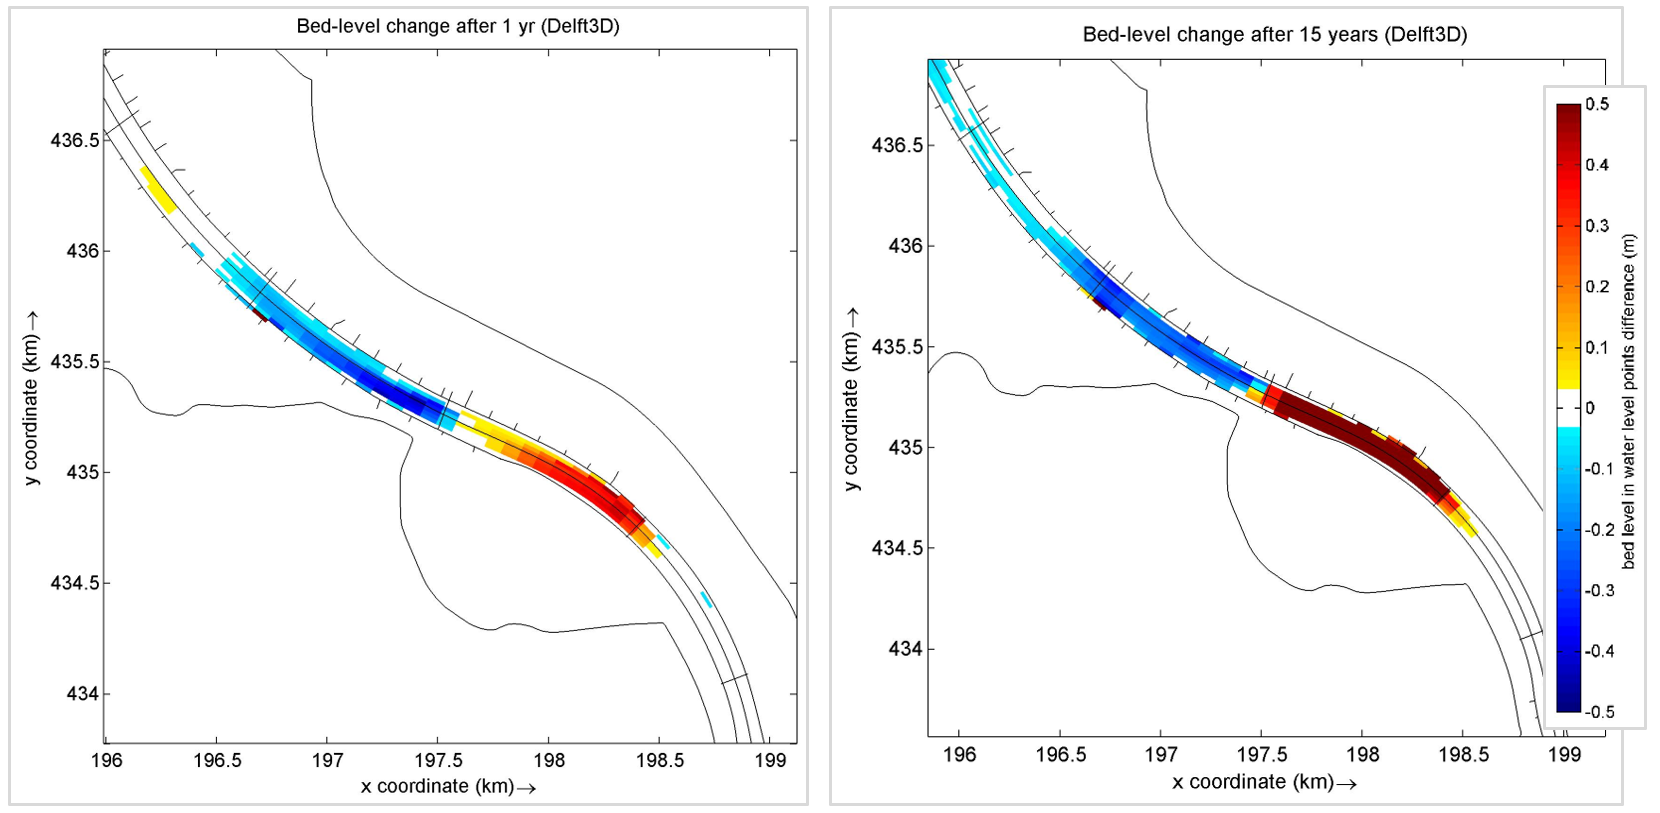
\includegraphics[width=\textwidth]{figures/Pannerden_mor.png}
\caption{The bed-level difference between the variant and the reference after 1 and 15 years of morphological simulation.}
\label{Pannerden_mor}
\end{figure}